\section{Set Theory}
Set theory is a foundational branch of mathematics that studies sets, which are simply collections of objects. At its core, it deals with the fundamental concepts of membership (whether an object belongs to a set), equality (when two sets are the same), and relationships between sets (like subsets, intersections, and unions).\\
It might seem simple, but set theory provides the basic language and tools to define and reason about almost all mathematical objects, from numbers and functions to more complex structures. It helps us understand the concept of infinity, organize mathematical ideas logically, and resolve paradoxes that arise from dealing with collections.\\
In essence, set theory provides the building blocks upon which much of modern mathematics is constructed.


\subsection{Basics}
To be concise, a set is a collection of mathematical objects that can also be other sets.\\
Here is a list of common symbols for set theory.

\begin{itemize}[label=\(-\)]
	\item \textbf{Empty set (\(\emptyset\))}: The set that contains no elements. It is the unique set with zero elements.

	\item \textbf{Example set with two elements}: A set that contains exactly two elements, such as \(\{1, 2\}\).

	\item \textbf{\(A \subseteq B\)}: Set \(A\) is a subset of \(B\). This means every element of \(A\) is also in \(B\).

	\item \textbf{\(A \subseteq B\) or \(A = B\)}: This notation already includes the possibility that \(A\) equals \(B\) since a set is always a subset of itself.

	\item \textbf{\(A \cup B\)}: The union of sets \(A\) and \(B\). It includes all elements that are in \(A\), in \(B\), or in both.

	\item \textbf{\(A \cap B\)}: The intersection of sets \(A\) and \(B\). It includes only the elements that are in both sets.

	\item \textbf{\(A \setminus B\)}: The difference of sets. Elements in \(A\) that are not in \(B\).

	\item \textbf{\(A^c\) or \(\overline{A}\)}: The complement of set \(A\). All elements not in \(A\), relative to a universal set.

	\item \textbf{\(|A|\)}: The cardinality of set \(A\), which is the number of elements in the set.
\end{itemize}

\smallskip
\subsubsection{Visuals}

\begin{figure}[H]
	\centering
	\begin{minipage}{0.45\textwidth}
		\centering
		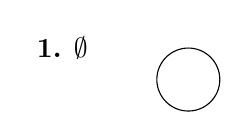
\begin{tikzpicture}[scale=0.8]
			% 1. Empty set
			\node at (0,0) {\textbf{1.} \(\emptyset\)};
			\draw (2,-0.5) circle (0.5);
		\end{tikzpicture}
		\caption*{1. Empty Set}
	\end{minipage}
	\hfill
	\begin{minipage}{0.45\textwidth}
		\centering
		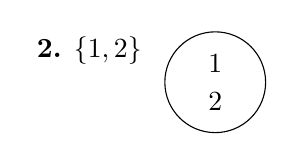
\begin{tikzpicture}[scale=0.8]
			% 2. Set with two elements
			\node at (0,0) {\textbf{2.} \(\{1,2\}\)};
			\draw (2,-0.5) circle (0.8);
			\node at (2,-0.2) {1};
			\node at (2,-0.8) {2};
		\end{tikzpicture}
		\caption*{2. Set with Two Elements}
	\end{minipage}

	\vspace{0.5cm}

	\begin{minipage}{0.45\textwidth}
		\centering
		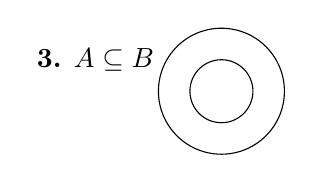
\begin{tikzpicture}[scale=0.8]
			% 3. A subset of B
			\node at (0,0) {\textbf{3.} \(A \subseteq B\)};
			\draw (2,-0.5) circle (1);
			\draw (2,-0.5) circle (0.5);
		\end{tikzpicture}
		\caption*{3. A is a subset of B}
	\end{minipage}
	\hfill
	\begin{minipage}{0.45\textwidth}
		\centering
		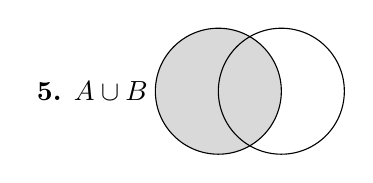
\begin{tikzpicture}[scale=0.8]
			% 5. Union
			\node at (0,0) {\textbf{5.} \(A \cup B\)};
			\begin{scope}
				\clip (2,0) circle(1);
				\fill[gray!30] (3,0) circle(1);
			\end{scope}
			\fill[gray!30] (2,0) circle(1);
			\draw (2,0) circle(1);
			\draw (3,0) circle(1);
		\end{tikzpicture}
		\caption*{5. Union of A and B}
	\end{minipage}

	\vspace{0.5cm}
\end{figure}

\newpage

\begin{figure}
	\centering
	\begin{minipage}{0.45\textwidth}
		\centering
		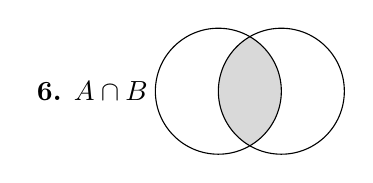
\begin{tikzpicture}[scale=0.8]
			% 6. Intersection
			\node at (0,0) {\textbf{6.} \(A \cap B\)};
			\begin{scope}
				\clip (2,0) circle(1);
				\fill[gray!30] (3,0) circle(1);
			\end{scope}
			\draw (2,0) circle(1);
			\draw (3,0) circle(1);
		\end{tikzpicture}
		\caption*{6. Intersection of A and B}
	\end{minipage}
	\hfill
	\begin{minipage}{0.45\textwidth}
		\centering
		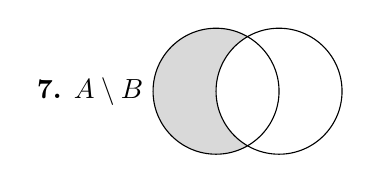
\begin{tikzpicture}[scale=0.8]
			% 7. A \ B
			\node at (0,0) {\textbf{7.} \(A \setminus B\)};
			\fill[gray!30] (2,0) circle(1);
			\begin{scope}
				\clip (3,0) circle(1);
				\fill[white] (2,0) circle(1);
			\end{scope}
			\draw (2,0) circle(1);
			\draw (3,0) circle(1);
		\end{tikzpicture}
		\caption*{7. A minus B}
	\end{minipage}

	\vspace{0.5cm}

	\begin{minipage}{0.45\textwidth}
		\centering
		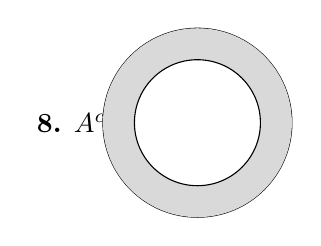
\begin{tikzpicture}[scale=0.8]
			% 8. Complement
			\node at (0,0) {\textbf{8.} \(A^c\)};
			\draw (2,0) circle(1.5);
			\fill[gray!30] (2,0) circle(1.5);
			\fill[white] (2,0) circle(1);
			\draw (2,0) circle(1);
		\end{tikzpicture}
		\caption*{8. Complement of A}
	\end{minipage}
\end{figure}
\smallskip

\subsection{Axioms of Set Theory (Zermelo Fraenkel)}
\smallskip
This are Zermelo Fraenkel axioms of set theory including \textit{The Axiom of Choice}.

\begin{enumerate}[label = \Roman*.]
	\item \textbf{Axiom of Extensionality:} \quad \(\forall A, B: A = B \Rightarrow (\forall C: C \in A \Leftrightarrow C \in B)\)
	\item \textbf{Empty-Set Axiom:} \quad \(\exists \emptyset : \forall X: X \notin \emptyset\)
	\item \textbf{Axiom of Pairing:} \quad \(\forall A, B: \exists C: \forall D: D \in C \Leftrightarrow (D = A \lor D = B)\)
	\item \textbf{Axiom of Union:} \quad \(\forall A: \exists B: \forall C: C \in B \Leftrightarrow (\exists D: C \in D \land D \in A)\)
	\item \textbf{Axiom of Infinity:} \quad \(\exists N: \emptyset \in N \land (\forall x: x \in N \Rightarrow x \cup \{x\} \in N)\)
	\item \textbf{Axiom Schema of Specification:} \quad \(\forall A: \exists B: \forall C: C \in B \Leftrightarrow (C \in A \land P(C))\)
	\item \textbf{Axiom Schema of Replacement:} \quad \(\forall A: \exists B: \forall y: y \in B \Rightarrow \exists x \in A: y = F(x)\)
	\item \textbf{Powerset Axiom:} \quad \(\forall A: \exists B: \forall C: C \subseteq A \Rightarrow C \in B\)
	\item \textbf{Foundation Axiom:} \quad \(\forall A \ne \emptyset: \exists B \in A: A \cap B = \emptyset\)
	\item \textbf{Axiom of Choice:} \quad \(\forall X:
		      \left( \left[ \forall A \in X: A \ne \emptyset \right] \land
		      \left[ \forall B, C \in X: B \ne C \Rightarrow B \cap C = \emptyset \right] \right) \\
		      \qquad \Rightarrow \exists Y: \forall I \in X: \exists! J \in Y: J \in I\)
\end{enumerate}

\subsection{The Cartesian Product}

The Cartesian product of two sets \(A\) and \(B\), written \(A \times B\), is the set of all ordered pairs in which the first element belongs to \(A\) and the second belongs to \(B\):
\[A \times B = \{ (a, b) : a \in A, \land\ b \in B\}.\]

\textbf{Example:}
\begin{table}[H]
	\centering
	\caption{Cartesian Product of \(A = \{1, 2, 3\}\) and \(B = \{4, 5, 6\}\)}
	\begin{tabular}{|c|c|c|c|}
		\hline
		\multirow{3}{*}{\(A \times B\)} & \multicolumn{3}{c|}{\(b \in B\)}                       \\
		\cline{2-4}
		                              & \(4\)                            & \(5\)      & \(6\)      \\
		\hline
		\(a \in A\)                     &                                &          &          \\
		\hline
		\(1\)                           & \((1, 4)\)                       & \((1, 5)\) & \((1, 6)\) \\
		\hline
		\(2\)                           & \((2, 4)\)                       & \((2, 5)\) & \((2, 6)\) \\
		\hline
		\(3\)                           & \((3, 4)\)                       & \((3, 5)\) & \((3, 6)\) \\
		\hline
	\end{tabular}
	\label{tab:cartesian_product}
\end{table}

The general cartesian product of \textit{n} sets can be written as:
\begin{align*}
	X_{i = 1}^{n + 1} A_i & = \left( X_{i = 1}^{n} A_i \right) \times A_{n + 1} \quad \text{with} \quad X_{i = 1}^{1} A_i = A_1 \\
	\text{When } A_i      & = M \ \text{for all } i:                                                                            \\
	M^n                   & := M \times M \times \cdots \times M = X_{i = 1}^{n} M \quad \text{with} \quad M^1 = M
\end{align*}

\subsection{Laws of Set Algebra}
Let \(X\) be the universal set and \(A, B, C \subseteq X\).

\begin{itemize}[label=\(-\)]
	\item \(\emptyset \subseteq A\)
	\item \(A \subseteq B \iff A \cap B = A \iff A \cup B = B \iff X \setminus B \subseteq X \setminus A \iff B \subseteq A\)
	\item \(A \cup B = B \cup A\) \hfill (Commutative Law)
	\item \(A \cap B = B \cap A\) \hfill (Commutative Law)
	\item \((A \cup B) \cup C = A \cup (B \cup C)\) \hfill (Associative Law)
	\item \((A \cap B) \cap C = A \cap (B \cap C)\) \hfill (Associative Law)
	\item \(A \cap (B \cup C) = (A \cap B) \cup (A \cap C)\) \hfill (Distributive Law)
	\item \(A \cup (B \cap C) = (A \cup B) \cap (A \cup C)\) \hfill (Distributive Law)
	\item \(A \cup A = A \quad \text{and} \quad A \cap A = A\) \hfill (Idempotent Law)
	\item \(A \setminus B = A \cap (X \setminus B) = A \cap \overline{B}\)
	\item \(B = \overline{A} \iff (A \cup B = X \land A \cap B = \emptyset)\) \hfill (Disjoint Partition of \(X\))
	\item \(\overline{A} \cap \overline{B} = \overline{A \cup B}\) \hfill (De Morgan's Law)
	\item \(\overline{A} \cup \overline{B} = \overline{A \cap B}\) \hfill (De Morgan's Law)
	\item \(\overline{\overline{A}} = A\) \hfill (Double Negation)
\end{itemize}

\subsubsection{Proof of De Morgans's Law for sets and logic}
The complement of \( A \cup B \) is \( \overline{(A \cup B)} \), and Law (11) on disjoint decomposition states:
\[
	B = \overline{A} \iff (A \cup B = X) \land (A \cap B = \emptyset)
\]

So define \( \overline{C} := A \cup B \) and \( D := \overline{A} \cap \overline{B} \),
and use Law (11) to show the disjoint decomposition:
\[
	D = C \iff A \cap B = A \cup B
\]

\textbf{a To show:}
\[
	D \cup C = X \iff (\overline{A} \cap \overline{B}) \cup (A \cup B) = X
\]

\begin{align*}
	(\overline{A} \cap \overline{B}) \cup (A \cup B)
	 & = (\overline{A} \cup A \cup B) \cap (\overline{B} \cup A \cup B) \quad \text{(Law (8))} \\
	 & = (X \cup B) \cap (X \cup A)                                                            \\
	 & = X \cap X                                                                              \\
	 & = X
\end{align*}

\textbf{b To show:}
\[
	D \cap C = \emptyset \iff (\overline{A} \cap \overline{B}) \cap (A \cup B) = \emptyset
\]

\begin{align*}
	(\overline{A} \cap \overline{B}) \cap (A \cup B)
	 & = (A \cap B \cap A) \cup (A \cap B \cap B) \quad \text{(Law (7))}                      \\
	 & = (\overline{A} \cap A \cap \overline{B}) \cup (\overline{A} \cap \overline{B} \cap B) \\
	 & = (\emptyset \cap \overline{B}) \cup (\overline{A} \cap \emptyset)                     \\
	 & = \emptyset \cup \emptyset                                                             \\
	 & = \emptyset
\end{align*}

\subsection{Indexed Sets}
Let \( X \) be a set, and \( A_i \subseteq X \) for all \( i \in J \), where \( J \) is the index set.

\textbf{a If \( J = \{1, 2, \dots, n\} \):}
\[
	\bigcup_{i=1}^{n} A_i := A_1 \cup A_2 \cup \dots \cup A_n = \{ x \mid \exists i \in J \ (x \in A_i) \}
\]
\[
	\bigcap_{i=1}^{n} A_i := A_1 \cap A_2 \cap \dots \cap A_n = \{ x \mid \forall i \in J \ (x \in A_i) \}
\]
\[
	X_{i=1}^{n} A_i = \{(a_1, \dots, a_n) \mid a_i \in A_i \}
\]

\textbf{b If \( J \) is any set:}
\[
	\bigcup_{i \in J} A_i := \{ x \mid \exists i \in J \ (x \in A_i) \}
\]
\[
	\bigcap_{i \in J} A_i := \{ x \mid \forall i \in J \ (x \in A_i) \}
\]

\textbf{c If \( J \) is any set, then \( (A_i)_{i \in J} \) are pairwise disjoint if and only if:}
\[
	\forall i_1, i_2 \in J, \ i_1 \neq i_2 \Rightarrow A_{i_1} \cap A_{i_2} = \emptyset
\]

\textbf{d If \( J \) is any set, then \( (A_i)_{i \in J} \) forms a (disjoint) decomposition of \( X \) if and only if:}
\[
	(A_{i})_{i \in J} \text{ are pairwise disjoint and } \bigcup_{i \in J} A_i = X
\]

\subsubsection{More Partitions Laws}
Let \( A_i, B_j \subseteq X \) for \( i \in I \) and \( j \in J \). Then the following holds:

\begin{itemize}[label=\(-\)]


	\item\textbf{De Morgan's Laws:}
	\[
		\overline{\bigcap_{i \in I} A_i}= \bigcup_{i \in I} \overline{A_i} \quad \text{and} \quad \overline{\bigcup_{i \in I} A_i} = \bigcap_{i \in I} \overline{A_i}
	\]

	\item\[
		\bigcap_{i \in I} A_i \cup \bigcap_{j \in J} B_j = \bigcap_{i,j} (A_i \cup B_j) \quad \text{with} \quad \bigcap_{i,j} = \bigcap_{(i,j) \in I \times J}
	\]


	\item\[
		\bigcup_{i \in I} A_i \cap \bigcup_{j \in J} B_j = \bigcup_{i,j} (A_i \cap B_j) \quad \text{with} \quad \bigcup_{i,j} = \bigcup_{(i,j) \in I \times J}
	\]

\end{itemize}
Here, \( I = \{ 1, 2, 3, \dots, n \} \) and \( J = \{ 1, 2, 3, \dots, m \} \). Then:
\[
	I \times J = \{ (i, j) \mid 1 \leq i \leq n, 1 \leq j \leq m, i, j \in \mathbb{N} \}
\]
\[
	= \{ (1, 1), (1, 2), \dots, (1, m), (2, 1), (2, 2), \dots, (2, m), \dots, (n, 1), (n, 2), \dots, (n, m) \}
\]

\subsection{Cardinality}
The cardinality of a set is the number of elements in that set.

Let \( A \) and \( B \) be finite sets with \( |A| = n \), \( |B| = m \), and let \( X \) be the finite universal set. Then the following holds:

\textbf{Cardinality of a Set}
\[
	A = (A \cap B) \cup (A \setminus B), \quad |A| = |A \cap B| + |A \setminus B|
\]

\textbf{Cardinality of the complements}
\[
	|A| = |X \setminus A| = |X| - |A|
\]
\[
	A \setminus B = A \cap (X \setminus B), \quad |A \setminus B| = |A| - |A \cap B|
\]

\textbf{Cardinality of the Cartesian Product}
\[
	|A \times B| = |A| \cdot |B| = n \cdot m
\]

\textbf{Inclusion-Exclusion Formula for Two Disjoint Sets}
\[
	|A \cup B| = |A| + |B| = n + m
\]

\textbf{Inclusion-Exclusion Formula for Two Non-Disjoint Sets}
Let \( |A \cap B| = k \), then:
\[
	|A \cup B| = |A| + |B| - |A \cap B| = n + m - k \quad \text{(since we do not count the intersection twice)}
\]

\textbf{Inclusion-Exclusion Formula for Three Non-Disjoint Sets}
\[
	|A \cup B \cup C| = |(A \cup B) \cup C| = |A \cup B| + |C| - |(A \cup B) \cap C|
\]
\[
	= |A| + |B| - |A \cap B| + |C| - |(A \cap C) \cup (B \cap C)|
\]
\[
	= |A| + |B| + |C| - |A \cap B| - |A \cap C| - |B \cap C| + |A \cap B \cap C|
\]

\subsubsection{General Formula for the cardinality of the union of sets}

\[
	\left\vert \bigcup_{i = 1}^n M_i \right\vert  = \sum_{I \subseteq \{1, \dots, n\}, I \neq \emptyset}(-1)^{|I| - 1} \left\vert \bigcap_{i \in I} M_i \right\vert
\]

\subsection{The Power Set}
The Power Set of a set is the set of all subsets of a given set \[
	P(x):= \{ M: M \subset X\}
\]
Its cardinality is \(2^n\) with \textit{n} being the number of elements in the original set \textit{X}.

\subsection{Family of Subsets}
Let \textit{X} be a non empty set. A subset \(\mathscr{F}\) of the power set of \textit{X} is called a set system of \textit{X}

\subsection{Partition}
Let \textit{X} be a non empty set. A subset \(\mathscr{F}\) of the power set of \textit{X} is called a partition if:\\
- \(M \neq  \emptyset\ \forall M \in \mathscr{F}\)\\
- \(\bigcap \mathscr{F} = X\)\\
- \(M_1 \bigcap M_2 \ne \emptyset \implies M_1 = M_2\ \forall\ M_1, M_2 \in \mathscr{F} \)

\begin{itemize}[label=\(-\)]

	\item Every equivalence relation corresponds to a partition:
	      \[
		      J: \{ R : R\ \text{is an equivalence relation on } X\} \to \{ F: F\ \text{is a partition of } X\}
	      \]

	      where \( J(R) := X / R \) is a bijection.

	\item If \( F \) is a partition of \( X \), then we can define an equivalence relation \( R_F \) by:
	      \[
		      R_F := \{ (x, y) \in X \times X : \exists M \in F\ \text{such that } x, y \in M \}
	      \]
	      Then \( R_F \) is an equivalence relation on \( X \).

\end{itemize}


\subsection{Family of Subsets Operations}
Let \(\mathscr{F}\) be a system of sets (a family of subsets) on the set \( X \). We define:

\[
	\bigcup_{M \in F} M := \bigcup F := \{ x \in X : \text{there exists } M \in F \text{ such that } x \in M \} ,
\]

\[
	\bigcap_{M \in F} M := \bigcap F := \{ x \in X : x \in M \text{ for all } M \in F \} .
\]
\newpage